% =========================================================
% CSC311 Final Project Report -- Group 65254
% Rebuilt from report.pdf (commit c6b789a) on the course template,
% with the boundary-check figure and paragraphs added.
% Single column, 12pt, 8 pages max.
% =========================================================

\documentclass[12pt]{article}

% ---------- Packages ----------
\usepackage[margin=1in]{geometry}
\usepackage{parskip}
\usepackage{graphicx}
\usepackage{booktabs}
\usepackage{amsmath, amssymb}
\usepackage{siunitx}
\usepackage[hidelinks]{hyperref}
\usepackage{caption}
\usepackage{enumitem}
\usepackage{xcolor}
\usepackage{XCharter}
\usepackage[xcharter]{newtxmath}
\usepackage[scaled=0.96]{inconsolata}

%--------- Headers and footers ------
\usepackage{fancyhdr}
\pagestyle{fancy}
\setlength{\headheight}{14.49998pt}
\fancyhf{}
\fancyhead[L]{CSC311 Project Report}
\fancyhead[R]{Group 65254}
\fancyfoot[C]{\thepage}

% ---------- Captions & Lists ----------
\captionsetup{font=small, labelfont=bf}
\setlist[itemize]{noitemsep, topsep=2pt}
\setlist[enumerate]{noitemsep, topsep=2pt}

\newcommand{\knn}{$k$NN}

\begin{document}

% =========================================================
% Title Page
% =========================================================
\begin{titlepage}
    \centering
    \vspace*{3cm}

    {\Large {CSC311: Introduction to Machine Learning} \par}
    \vspace{1cm}

    {\Large {Project Report} \par}
    \vspace{1cm}

    {\large \textit{Sport Classification from Survey Responses} \par}
    \vspace{3cm}

    {\large Submitted by \par}

    \vspace{0.5cm}
    {\large Group 65254}

    \vspace{0.5cm}
    {\large Chuning Li, Shimeng Wang, Yihe Xiao, Jiaqi Zhao \par}

    \vfill
    {\large University of Toronto \\ Fall 2026 \par}
\end{titlepage}
\clearpage
\setcounter{page}{1}

% ================================================
% 1. Executive Summary
% ================================================
\section{Executive Summary}

We compared $k$-nearest neighbours, an entropy decision tree, and
L2-regularized softmax regression on a three-class sport survey. The tuned
L2-regularized softmax model was selected by macro-F1 on held-out student
respondents and refitted on all development respondents. Its projected
accuracy is 91.67\%, using accuracy on a separate internal test as a proxy for
the unseen instructor/TA set. Combining evidence across questions appears to
have helped it classify more consistently than a local vote or a single tree.

% ================================================
% 2. Data Exploration
% ================================================
\section{Data Exploration}\label{sec:data-exploration}

The 870 rows cover 290 respondents, with one Baseball, Basketball and Soccer
response per respondent. We reproduced the proposal split by sorting IDs,
shuffling with NumPy's default random generator at seed 42, and taking 203, 43
and 44 respondents for training, validation and internal test (609, 129 and 132
rows). We set the internal test aside before exploration. Grouping keeps a
person's wording and response habits within one partition. ID and label are
excluded from the predictors. Training has 203 rows per class, so no
rebalancing was applied and a constant prediction has 33.3\% accuracy.

\begin{table}[h]
\centering
\small
\begin{tabular}{llrl}
\toprule
Feature & Type & Missing & Training distribution (nonmissing) \\
\midrule
Ease of entry         & Numeric      & 4 (0.66\%)  & 13 values across 0--10, including fractions \\
Strategy              & Likert       & 5 (0.82\%)  & 5 levels, 49.0\% Agree \\
Injury risk           & Likert       & 4 (0.66\%)  & 5 levels, 38.0\% Agree \\
Individual brilliance & Likert       & 5 (0.82\%)  & 5 levels, 36.8\% Agree \\
Playing location      & Multi-select & 4 (0.66\%)  & 54 option combinations \\
Playing season        & Multi-select & 4 (0.66\%)  & 13 option combinations \\
Music                 & Multi-select & 4 (0.66\%)  & 96 option combinations \\
Food and drinks       & Text         & 10 (1.64\%) & 435 distinct answers \\
Colour                & Text         & 5 (0.82\%)  & 141 distinct answers \\
Song                  & Text         & 24 (3.94\%) & 348 distinct answers \\
Viewing feelings      & Text         & 4 (0.66\%)  & 329 distinct answers \\
Ticket price          & Numeric text & 4 (0.66\%)  & 231 answer patterns, 555 parsed rows \\
\bottomrule
\end{tabular}
\caption{Missingness and variation across 609 training rows. The price count
records explicit missing markers. A further 50 responses could not be parsed.}
\label{tab:features}
\end{table}

We lowercased responses, normalized whitespace and mapped explicit markers such
as \texttt{n/a}, \texttt{null}, \texttt{-} and \texttt{[]} to missing.
Meaningful responses such as \emph{none} were retained. No training rows were
exact duplicates and no respondent repeated a label. Two repeated
answer--label combinations across people were retained. Every nonmissing
training rating and Likert response was valid.

\subsection*{Preprocessing and observed class relationships}

We treated bare amounts and unspecified dollar signs as CAD, extracted single
amounts and stated caps, and took the midpoint of simple ranges. Explicit
foreign currencies and ambiguous or unsupported forms were left missing. Of 609
prices, 555 parsed successfully (91.1\%). Parsed class medians were CAD 50, 150
and 150 for Baseball, Basketball and Soccer. Means were CAD 86, 224 and 309,
reflecting a long right tail. We kept prices above the training IQR upper fence
of CAD 425 and applied $\log(1+\text{price})$ to reduce their influence.

Ease ratings were bounded at 0--10 and Likert answers were mapped from strongly
disagree (1) to strongly agree (5), assuming equal spacing. Numeric and ordinal
inputs were median-imputed on their original scales, then standardized after
the price log transform using the fitted mean and population standard
deviation. Scaling matters for Euclidean distance and the relative effect of a
shared L2 penalty. Each observed multi-select option became a binary
indicator. We ignored unseen options and added one missingness flag for each of
the 12 questions. Invalid numeric and ordinal answers trigger their flags.

Missingness was related to the label. Soccer responses had no missing values
except for one song answer (0.99\%), whereas Baseball and Basketball responses
were missing 1--6\% of answers per question, most often for song and food. This
supported a missingness flag for every question rather than silent imputation.
Spearman correlations between the five numeric and ordinal features were all
below 0.33 in absolute value (largest: strategy and injury risk, 0.32), so no
pair was redundant and all were kept. No encoded feature was constant on the
training split; the least varied features still took two distinct values.

We fitted separate unigram TF-IDF vocabularies for food, colour, song and
feelings. Terms occur in at least the configured number of fitting documents,
with at most 100 terms per field. For each response we multiplied term counts
by smoothed IDF, $\log((1+n)/(1+\mathrm{df}))+1$, and L2-normalized the field
vector~\cite{skl-tfidf}. Missing responses have zero text vectors and unseen
tokens are ignored. Binary and text features keep their native scales in the
proposal representation. The starting minimum document frequency of two
yielded 390 features for 609 training rows.

\begin{table}[h]
\centering
\small
\begin{tabular}{lrrrl}
\toprule
Sport & Mean ease & Winter selected & Summer selected & Top colour token \\
\midrule
Baseball   & 4.13 & 6.9\%  & 91.6\% & blue \\
Basketball & 5.96 & 57.1\% & 92.1\% & orange \\
Soccer     & 6.19 & 8.4\%  & 92.6\% & green \\
\bottomrule
\end{tabular}
\caption{Season percentages use all 203 training rows per class. The colour
token has the highest mean training TF-IDF within its class.}
\label{tab:class-relationships}
\end{table}

Winter selection was strongly associated with Basketball. Summer selection was
common across all classes and offered less separation. Mean ease was lower for
Baseball, but within-class standard deviations of 1.99--2.27 indicated overlap.
Baseball song responses prominently featured words from \emph{Take Me Out to
the Ball Game}. \emph{Waka} and \emph{shakira} stood out for Soccer.
\emph{Bored} led Baseball's feeling tokens by mean TF-IDF, while
\emph{excited} led both other sports. These associations motivated comparing a
model that combines word evidence across fields, a tree that can use seasonal
rules, and a neighbourhood model that can exploit similar answer profiles.

% ================================================
% 3. Methodology
% ================================================
\section{Methodology}\label{sec:methodology}

\subsection*{Models and optimization}

\textbf{$k$-nearest neighbours.} We stored training vectors and used uniform
voting among the $k$ nearest in Euclidean distance. Exact distance ties follow
training row order. Vote ties follow Baseball, Basketball, Soccer. Small $k$
retains local survey patterns but is noise-sensitive. Larger $k$ smooths the
vote. There is no gradient optimizer.

\textbf{Decision tree.} We used scikit-learn's entropy criterion with greedy
binary threshold splits, depth and minimum leaf-size constraints, and random
state 42. Leaves predict the most common class. The tree can represent
dependencies between venue, season and other features. Depth and leaf-size
controls constrain memorization of rare responses.

\textbf{L2-regularized softmax regression.} We used NumPy to minimize mean
multiclass cross-entropy plus $\lambda\|W\|_F^2/2$, excluding the bias. Scores
are $xW+b$. We initialized parameters to zero, used numerically stable
full-batch gradient descent at a constant step size, and stopped at 5,000
updates or after 20 consecutive updates with relative objective change below
$10^{-7}$. We logged losses at initialization, every 100 updates and at
termination. Nonfinite runs or objective increases beyond $10^{-12}$ made a
configuration ineligible. Finite, decreasing runs at the iteration cap were
flagged and remained eligible. This model combines sparse text and option
signals while L2 shrinkage controls large coefficients.

\subsection*{Response grouping and tuning}

At each minimum document frequency, we fitted preprocessing separately on the
fit portion of each of five training folds created with
GroupKFold~\cite{skl-groupkfold}. Medians, moments, option sets, text
vocabularies and IDF values came only from fold fitting rows. Every setting
used the same partitions. The 129 separate validation rows stayed aside until
each model family had a champion.

\begin{table}[h]
\centering
\small
\begin{tabular}{llr}
\toprule
Family & Parameters crossed with minimum document frequency in $\{2,3,5\}$ & Settings \\
\midrule
\knn    & $k\in\{1,3,5,9,15\}$ & 15 \\
Tree    & Depth $\in\{3,5,8,\text{None}\}$, leaf size $\in\{2,5,10\}$ & 36 \\
Softmax & Rate $\in\{0.01,0.05,0.10\}$, $\lambda\in\{10^{-4},10^{-3},10^{-2},10^{-1}\}$ & 36 \\
\midrule
\multicolumn{3}{l}{\emph{Training-only extensions}} \\
\knn    & $k\in\{1,3,5,9,15\}$, text weight $w\in\{0.5,2\}$ & 30 \\
Softmax & Rate $\in\{0.20,0.40\}$, $\lambda\in\{10^{-4},10^{-3},10^{-2},10^{-1}\}$ & 24 \\
\midrule
\multicolumn{3}{l}{\emph{Boundary check}} \\
\knn    & $k\in\{21,31,45\}$, $w\in\{0.5,1,2\}$ & 27 \\
Softmax & Rate $\in\{0.1,0.2,0.4\}$, $\lambda\in\{0,10^{-5},10^{-4}\}$, 20{,}000 updates & 27 \\
\bottomrule
\end{tabular}
\caption{The exhaustive proposal grid comprises 87 settings and 435 fold fits.
With the extensions and the boundary check, 195 settings and 975 fold fits
were evaluated on the same training folds.}
\label{tab:grid}
\end{table}

The $k$ grid ranges from highly local to smoother decisions on roughly 487
fitting rows per fold. Tree limits span shallow rules to unrestricted depth,
with minimum leaf sizes limiting rare branches. Penalties span three orders of
magnitude to address the high feature count. Multiple rates let us check
convergence. Minimum document frequency controls rare-word retention.

\subsection*{Training-only extensions and final selection}

On the same training folds, we crossed the original $k$ and
document-frequency choices with text-block multipliers 0.5 and 2 to test how
much text should contribute to Euclidean distance (30 extra settings). We also
crossed softmax rates 0.20 and 0.40 with the original penalties and document
frequencies to test whether faster objective descent helped under the fixed cap
(24 settings). All 270 extra fits preceded any held-out validation scoring.
The tree grid stayed as proposed. \knn{} proposal/expanded best CV macro-F1
was 81.9\%/88.1\%. Softmax proposal/expanded best CV macro-F1 was
89.3\%/89.3\%.

Two champions sat on the edge of their grids: \knn{} chose the largest $k$
(15), and softmax chose the smallest penalty ($\lambda=10^{-4}$) while stopping
at the 5,000-update cap. We therefore ran a boundary check on the same five
training folds (54 settings, 270 fold fits; Table~\ref{tab:grid}).
Figure~\ref{fig:tuning} shows the result. \knn{} macro-F1 peaks at $k=15$ and
falls for every larger $k$ (86.8\% at 21, 85.9\% at 45). Softmax is flat for
$\lambda\le 10^{-2}$ (88.8--89.3\%) and drops only at $\lambda=0.1$ (87.2\%).
Removing the penalty or training four times longer did not help: the best
boundary setting reached 89.1\%, below the 89.3\% champion. Stopping at 5,000
updates therefore acts as mild early stopping rather than as an optimization
failure. No boundary setting improved on its family's champion, so the
selected configurations were unchanged.

\begin{figure}[h]
  \centering
  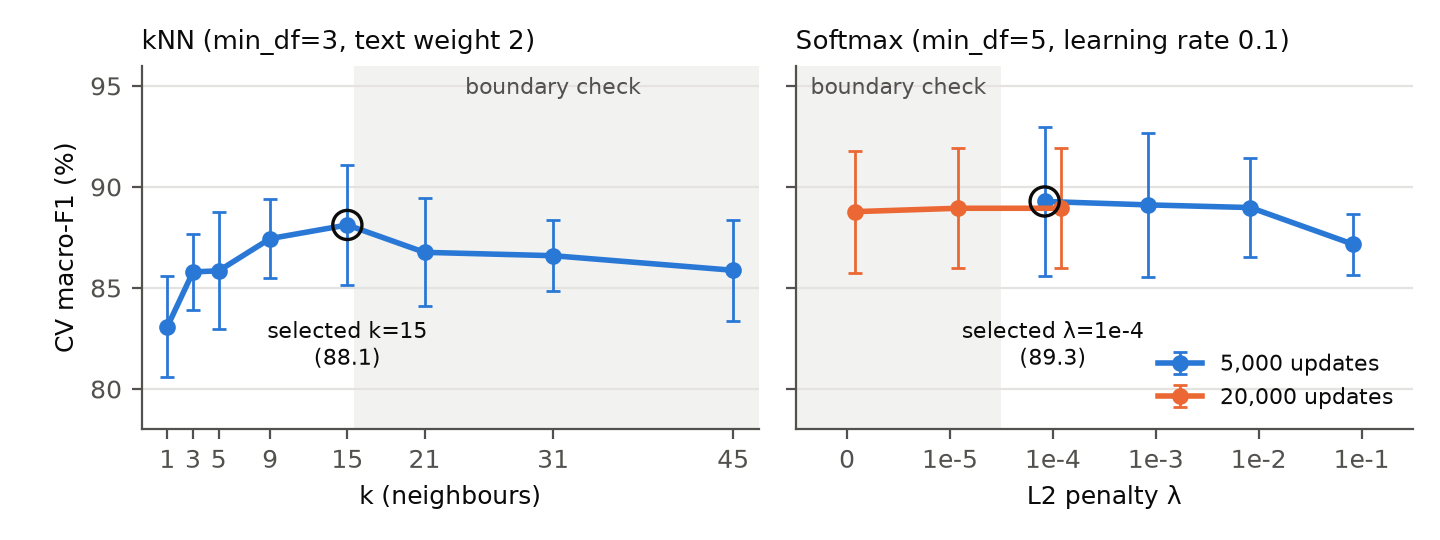
\includegraphics[width=\linewidth]{figures/tuning_curves.png}
  \caption{Mean grouped 5-fold CV macro-F1 (error bars: $\pm$1 sample SD
  across folds) for the selected representation of each family. The shaded
  region is the boundary check. Rings mark the selected settings. For
  softmax, blue points use the 5,000-update cap and orange points the
  20,000-update cap.}
  \label{fig:tuning}
\end{figure}

Within each family we maximized mean CV macro-F1, breaking exact ties by mean
accuracy, then larger $k$, shallower tree then larger leaves, or larger
$\lambda$, followed by fixed grid order. An extension could replace its
proposal champion only with a strict CV macro-F1 gain. We refitted each
champion on training and selected the family by held-out validation macro-F1,
with accuracy and serialized size as exact tie-breaks. The CV gap between
softmax and \knn{} (1.2 points) is smaller than either model's fold-to-fold
standard deviation (3.7 and 3.0 points), and softmax won only 3 of the 5 folds
(it beat the tree on 4 of 5). CV alone therefore does not separate these two
families, which is why the separate validation set makes the final choice. We
locked the configuration and refitted preprocessing and model parameters on
738 training-plus-validation rows. We scored the locked model once on the 132
internal test rows. The instructor/TA set remained unavailable.

\subsection*{Metrics and implementation}

Accuracy is the fraction of correct labels. Per-class precision is the fraction
of predictions for a sport that are correct. Recall is the fraction of that
sport's true responses identified. Class F1 is $2TP/(2TP+FP+FN)$, with zero
used for undefined ratios. Macro-F1 gives equal weight to each sport and
penalizes uneven performance even on a balanced dataset. Confusion matrices put
true sports in rows and predicted sports in columns. Row-normalization gives
recall on the diagonal and shows competing labels off the diagonal. CV sample
standard deviations describe variation across folds.

Development used Python, NumPy, pandas and scikit-learn~\cite{pedregosa2011}
for grouped folds, TF-IDF fitting and tree fitting. The proposal and
exploration code supplied the cleaning rules and split. Deployment uses
standard Python, NumPy and pandas. The prediction function applies exported
preprocessing and returns one sport string per CSV row without network access,
in accordance with the course requirements.

% ===========================================
% 4. Results
% ===========================================
\section{Results}\label{sec:results}

\begin{table}[h]
\centering
\small
\begin{tabular}{llrrrr}
\toprule
Family & Selected configuration & CV Acc. & CV F1 & Val.\ Acc. & Val.\ F1 \\
\midrule
\knn    & $k=15$, $d_f=3$, $w=2$ & 88.2 $\pm$ 2.9 & 88.1 $\pm$ 3.0 & 89.9 & 89.8 \\
Tree    & $d=8$, $\ell=2$, $d_f=5$ & 85.1 $\pm$ 1.6 & 85.0 $\pm$ 1.7 & 88.4 & 88.4 \\
Softmax & $\eta=0.10$, $\lambda=0.0001$, $d_f=5$ & 89.3 $\pm$ 3.6 & 89.3 $\pm$ 3.7 & 96.1 & 96.1 \\
\bottomrule
\end{tabular}
\caption{Metrics are percentages. CV shows mean $\pm$ sample SD over five
training folds. Validation uses 129 separate student responses. $d_f$ is
minimum document frequency and $w$ the text multiplier.}
\label{tab:family}
\end{table}

Softmax led held-out macro-F1 by 6.3 points over \knn. The softmax champion
reached its update cap after 5,000 updates on training, with no recorded
objective increases. The final refit reached the cap at 5,000 updates.

\begin{table}[h]
\centering
\small
\begin{tabular}{lrrrrrr}
\toprule
 & \multicolumn{2}{c}{Baseball} & \multicolumn{2}{c}{Basketball} & \multicolumn{2}{c}{Soccer} \\
\cmidrule(lr){2-3}\cmidrule(lr){4-5}\cmidrule(lr){6-7}
Split and model & P & R & P & R & P & R \\
\midrule
Validation \knn     & 88.9 & 93.0 & 89.1 & 95.3  & 92.1 & 81.4 \\
Validation Tree     & 81.2 & 90.7 & 93.0 & 93.0  & 92.1 & 81.4 \\
Validation Softmax  & 97.6 & 95.3 & 93.5 & 100.0 & 97.6 & 93.0 \\
Internal test       & 89.1 & 93.2 & 95.2 & 90.9  & 90.9 & 90.9 \\
\bottomrule
\end{tabular}
\caption{Precision (P) and recall (R), in percent, for each validation
champion and the final internal test.}
\label{tab:per-class}
\end{table}

\begin{table}[h]
\centering
\small
\setlength{\tabcolsep}{4pt}
\begin{tabular}{lrrrrrr}
\toprule
 & \multicolumn{3}{c}{Validation} & \multicolumn{3}{c}{Internal test} \\
\cmidrule(lr){2-4}\cmidrule(lr){5-7}
Actual sport & Base. & Bask. & Soc. & Base. & Bask. & Soc. \\
\midrule
Baseball   & 41 (95.3\%) & 1 (2.3\%)    & 1 (2.3\%)   & 41 (93.2\%) & 0 (0.0\%)   & 3 (6.8\%) \\
Basketball & 0 (0.0\%)   & 43 (100.0\%) & 0 (0.0\%)   & 3 (6.8\%)   & 40 (90.9\%) & 1 (2.3\%) \\
Soccer     & 1 (2.3\%)   & 2 (4.7\%)    & 40 (93.0\%) & 2 (4.5\%)   & 2 (4.5\%)   & 40 (90.9\%) \\
\bottomrule
\end{tabular}
\caption{Winner's confusion matrices. Columns are predictions. Cells show
count (row percentage).}
\label{tab:confusion}
\end{table}

Validation most common error (2 rows) involved Soccer predicted as
Basketball. Internal test most common errors (3 each) involved Baseball
predicted as Soccer and Basketball predicted as Baseball. Validation errors
affected 2/20 rows with missing or unparseable answers and 5/105 rows
containing unseen text tokens. These overlapping groups are descriptive.

Our single-number projection for instructor/TA test accuracy is 91.67\%, the
observed internal accuracy (121 of 132) after refit. Internal macro-F1 was
91.68\% and validation accuracy was 96.1\%. The holdout was grouped and
untouched until model lock; rerunning the pipeline with the boundary check
selected the same model with identical predictions. Student and instructor/TA
respondents may differ in wording and sport familiarity, so the projection uses
student data as a proxy and external accuracy remains unmeasured.

% ================================================
% 5. Contributions and Learning
% ================================================
\section{Contributions and Learning}

\begin{itemize}[itemsep=4pt]
  \item \textbf{Chuning Li.} I led survey cleaning and documented the
  preprocessing rules for all three models. I compared responses across sports
  to spot useful predictors and set rules for ambiguous ticket prices. I
  learned that even filling in missing values can leak information if the
  medians come from held-out responses, so we estimated them using training
  rows alone.
  \item \textbf{Shimeng Wang.} My focus was tuning k-nearest neighbours and the
  decision tree. I spent time comparing the sports each model confused on
  validation. Looking at those mistakes showed me how much class-by-class
  recall adds to a single accuracy score.
  \item \textbf{Yihe Xiao.} I worked on the softmax model, from trying learning
  rates and penalties to checking the saved prediction pipeline. What stuck
  with me was that the loss could keep falling all the way to the update limit
  without meeting our stopping rule.
  \item \textbf{Jiaqi Zhao.} I helped set up the respondent-level splits and
  organized the tuning results into tables. Putting the results side by side
  made it clear why I need to record which respondents and settings went into
  each run if I want someone else to reproduce it.
\end{itemize}

\textbf{AI assistance.} OpenAI ChatGPT (Codex) assisted with running model
comparisons and testing the prediction script on CSVs with blank answers and
unseen words.

% ==================================================
% 6. References
% ==================================================
\section{References}
{\renewcommand{\section}[2]{}% suppress thebibliography's own heading
\begin{thebibliography}{9}
\bibitem{skl-tfidf} The scikit-learn developers. \emph{TF-IDF term
weighting}. Scikit-learn 1.8.0 User Guide, 2025.
\bibitem{skl-groupkfold} The scikit-learn developers. \emph{GroupKFold}.
Scikit-learn 1.8.0 API Reference, 2025.
\bibitem{pedregosa2011} Fabian Pedregosa et al. \emph{Scikit-learn: Machine
Learning in Python}. Journal of Machine Learning Research, 12(85),
2825--2830, 2011.
\end{thebibliography}}

\end{document}
